\section*{Introduction} \label{sec:Introduction}


Cette tâche vise à explorer la compilation croisée en utilisant un compilateur dédié à l'architecture ARM et à l'exécution de programmes ARM sur un système x86\_64 à l'aide de l'émulateur QEMU. En combinant ces deux technologies, nous permettons le développement et le test de logiciels ARM sur des plates-formes x86\_64, offrant ainsi une solution pratique pour le développement embarqué et la compatibilité multiplateforme. Ce projet offre un aperçu détaillé de la compilation croisée, de l'émulation d'architecture, et des outils nécessaires pour travailler efficacement dans un environnement ARM, même sur un système hôte x86\_64.



\section{Mise à jour des référentiels APT}
\begin{figure}[h]
  
    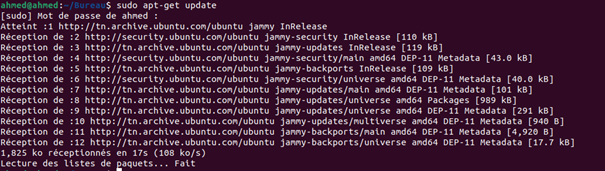
\includegraphics[width=1\textwidth]{images/Mise à jour des référentiels APT.png}
     
\end{figure}

\section{Installation des outils nécessaires, y compris le compilateur croisé pour ARM}

\begin{figure}[h]
  
    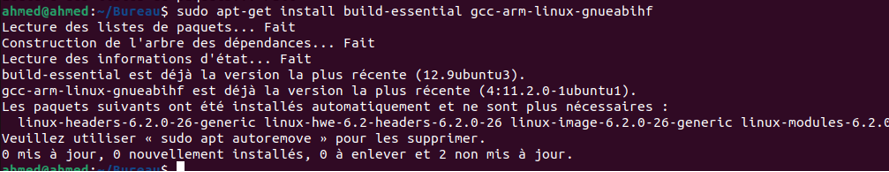
\includegraphics[width=1\textwidth]{images/outil.png}
   
\end{figure}

\section{Création d’un fichier hello.c  avec gedit}

\begin{figure}[h]

    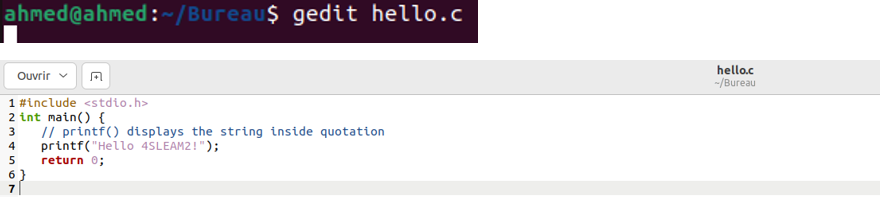
\includegraphics[width=0.8\textwidth]{images/1.png}

\end{figure}



\section{Compilation du fichier hello.c avec le compilateur croisé}

\begin{figure}[h]

    
\includegraphics[width=1\textwidth]{images/2.png}

\end{figure}
\section{Installation de l'émulateur QEMU pour exécuter le binaire ARM}
\begin{figure}[h]

    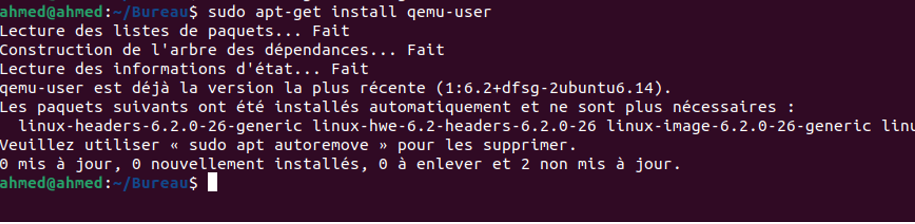
\includegraphics[width=1\textwidth]{images/3.png}

\end{figure}
QEMU (\textit{Quick EMUlator}) est un émulateur et un outil de virtualisation qui est souvent utilisé dans des projets tels que celui que vous avez décrit pour plusieurs raisons :
\begin{enumerate}
    \item \textbf{Émulation d'architecture :} QEMU est capable d'émuler différentes architectures matérielles, y compris l'architecture ARM. Cela signifie que vous pouvez exécuter des programmes destinés à ARM sur une machine x86\_64, ce qui est particulièrement utile pour le développement multiplateforme.
    \item \textbf{Facilité de configuration :} QEMU est relativement simple à installer et à configurer. Une fois que vous avez créé un environnement d'émulation ARM, il est facile d'y exécuter des binaires ARM sans avoir à déployer un matériel ARM réel.
    \item \textbf{Débogage :} QEMU offre des fonctionnalités de débogage puissantes, ce qui facilite le suivi et la résolution des problèmes dans les applications ARM sans avoir besoin d'un matériel ARM physique. Cela rend le développement et le test de logiciels plus pratiques.
    \item \textbf{Compatibilité :} QEMU est une solution bien établie et maintenue, ce qui signifie qu'elle est compatible avec de nombreuses distributions Linux et versions d'ARM, garantissant ainsi une grande flexibilité et une large base d'utilisateurs.
    \item \textbf{Performance raisonnable :} Bien que l'émulation soit généralement plus lente que l'exécution native, QEMU offre des performances suffisantes pour de nombreux cas d'utilisation de développement et de test, ce qui en fait un choix viable.
\end{enumerate}
\section{Création d’un lien symbolique pour le fichier ld-linux-armhf.so.3}
\begin{figure}[h]

    
\includegraphics[width=1\textwidth]{images/4.png}

\end{figure}
On a créé un lien symbolique vers le fichier ld-linux-armhf.so.3 pour résoudre un problème de compatibilité d'architecture lors de l'exécution de programmes ARM sur une machine x86\_64 à l'aide de l'émulateur QEMU.

\section{Définir la variable LD\_LIBRARY\_PATH }
\begin{figure}[h]

    
\includegraphics[width=1\textwidth]{images/5.png}

\end{figure}    
\section{Exécution du binaire ARM avec QEMU}
\begin{figure}[h]

    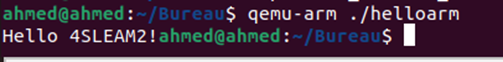
\includegraphics[width=0.8\textwidth]{images/7.png}

\end{figure}

\section{ Analyse du Fichier "helloarm" avec la Commande file}
\begin{figure}[h]

    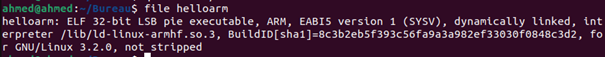
\includegraphics[width=1\textwidth]{images/6.png}

\end{figure}
La commande \texttt{file} permet d'obtenir des informations sur un fichier. Dans le cas de la commande \texttt{file helloarm}, elle retourne des informations sur le type de fichier, l'architecture cible, le système d'exploitation, etc.

Voici la décomposition des informations fournies :

\begin{itemize}
    \item \texttt{ELF 32-bit LSB ple executable} : Indique que le fichier est un fichier exécutable (ELF = Executable and Linkable Format) en 32 bits, utilisant un byte order (byte ordering) little-endian.
    \item \texttt{ARM, EABI version 1 (SYSV)} : Le fichier est conçu pour être exécuté sur une architecture ARM (Advanced RISC Machine), conformément à la version 1 de l'EABI (Embedded Application Binary Interface) et en utilisant le système d'exploitation SYSV (System V).
    \item \texttt{dynamically linked} : Le fichier contient des références à des bibliothèques externes, ce qui signifie qu'il faut d'abord charger ces bibliothèques pour exécuter le fichier.
    \item \texttt{interpreter /lib/ld-linux-armhf.so.3} : Le programme qui charge et exécute les dépendances dynamiques est /lib/ld-linux-armhf.so.3.
    \item \texttt{BuildID [sha1]=8c3b2eb5f393c56fa9a3a982ef33030f0848c3d2} : Un identifiant unique du fichier, calculé à l'aide de l'algorithme de hachage SHA-1.
    \item \texttt{for GNU/Linux 3.2.0} : Indique que le fichier a été compilé pour le système d'exploitation GNU/Linux, version 3.2.0.
    \item \texttt{not stripped} : Signifie que le fichier n'a pas été "strippé" (un processus qui supprime les informations de débogage pour réduire la taille du fichier et protéger le code source).
\end{itemize}

En somme, le fichier \texttt{helloarm} est un fichier exécutable en 32 bits pour une architecture ARM, compatible avec le système d'exploitation GNU/Linux 3.2.0 et utilisant l'EABI version 1 (SYSV). Il est compilé en utilisant le compilateur GNU/Linux.
\section*{Conclusion}
En conclusion, cette tâche "Cross-Compilation and ARM Emulation with QEMU" a permis d'explorer les concepts essentiels de la compilation croisée et de l'émulation d'architecture ARM sur des systèmes x86\_64. Grâce à l'utilisation d'un compilateur croisé, nous avons pu compiler des programmes spécifiques à l'architecture ARM sur un système hôte x86\_64. L'intégration de l'émulateur QEMU a ensuite permis d'exécuter ces programmes ARM avec succès, créant ainsi un environnement de test et de développement pratique pour les applications ARM.